\documentclass{tufte-handout}

%\geometry{showframe}% for debugging purposes -- displays the margins

\usepackage{amsmath}

% Set up the images/graphics package
\usepackage{graphicx}
\setkeys{Gin}{width=\linewidth,totalheight=\textheight,keepaspectratio}
\graphicspath{{graphics/}}

\title{Endocrine Control Systems}
\author{Dave Bridges}
%\date{24 January 2009}  % if the \date{} command is left out, the current date will be used

% The following package makes prettier tables.  We're all about the bling!
\usepackage{booktabs}

% The units package provides nice, non-stacked fractions and better spacing
% for units.
\usepackage{units}

% The fancyvrb package lets us customize the formatting of verbatim
% environments.  We use a slightly smaller font.
\usepackage{fancyvrb}
\fvset{fontsize=\normalsize}

% Small sections of multiple columns
\usepackage{multicol}

% Provides paragraphs of dummy text
\usepackage{lipsum}

% These commands are used to pretty-print LaTeX commands
\newcommand{\doccmd}[1]{\texttt{\textbackslash#1}}% command name -- adds backslash automatically
\newcommand{\docopt}[1]{\ensuremath{\langle}\textrm{\textit{#1}}\ensuremath{\rangle}}% optional command argument
\newcommand{\docarg}[1]{\textrm{\textit{#1}}}% (required) command argument
\newenvironment{docspec}{\begin{quote}\noindent}{\end{quote}}% command specification environment
\newcommand{\docenv}[1]{\textsf{#1}}% environment name
\newcommand{\docpkg}[1]{\texttt{#1}}% package name
\newcommand{\doccls}[1]{\texttt{#1}}% document class name
\newcommand{\docclsopt}[1]{\texttt{#1}}% document class option name

\begin{document}

\maketitle% this prints the handout title, author, and date

\begin{abstract}
\noindent This lecture covers general principles of endocrine control systems.  This lecture covers the following pages in the textbook: 12; 121-124; 319-332 \cite{Widmaier2013}
\end{abstract}

\section{Learning Objectives}
\begin{itemize}
\item Define endocrine, paracrine, autocrine, and exocrine systems, define neuro-secretory cells by giving a few examples.
\item List major categories of hormones and give several examples that belong to each class.
\item List important factors that determine hormone levels in circulation.
\item Describe four general functions of hormones.
\item Explain with examples neuroendocrine integration.
\item Explain cellular actions of hormones via membrane receptors.
\item Explain cellular action of hormones via protein synthesis.
\item Discuss major categories of cellular signal pathways of hormones via membrane receptors.
\item Discuss major categories of cellular signal pathways of hormones via cytosolic/nuclear receptors.
\item Define basal secretion and stimulated secretion of endocrine glands.
\item Describe negative and positive feedback system using an example.
\end{itemize}

\section{General Hormonal Principles}
\newthought{A major advantage of multicellularity}, is that biological roles are divided into specialized organs and tissues.  In a single cellular organism, such as \textit{Saccharomyces cerevisiae}\sidenote{also known as brewer's yeast}, all cells need to autonomously be able to sense the environment, cellular conditions and respond appropriately.  Multicellular organisms are able to use more sophisticated mechanisms to sense the environment and make these decisions.  Essential to this division of labor is the ability of these organ systems to communicate efficiently and effectively with each other.  This is accomplished through hormones, which are secreted from one organ to another.

\subsection{Hormonal Classification}

There are hundreds, if not thousands hormones, if defined loosely to mean \emph{chemicals derived from one cell that can affect another cell}.  Remembering what these all do, how they are made, where they come from can be a challenge.  To simplify this, these can be grouped several ways including chemically, anatomically or functionally.  

\newthought{Chemically,} hormones can be small molecules such as amino acids or lipids, or can be small polypeptides, or even large proteins with three dimensional structures (see Figure \ref{fig:chemical-classification}).  Often, an endocrine organ only releases hormones of a particular chemical class.  An example of this is the adrenal gland which secretes several steroid hormones, each of which have different roles and target tissues.

\begin{marginfigure}
  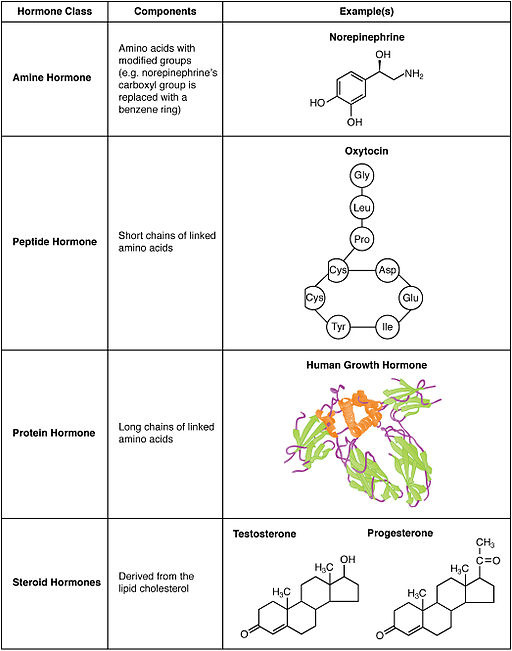
\includegraphics{figures/hormone-classification}
  \caption{Chemical classification of hormones.  From Anatomy \& Physiology, Connexions Web site. http://cnx.org/content/col11496/1.6/, Jun 19, 2013. OpenStax College.}
    \label{fig:chemical-classification}
\end{marginfigure}

\newthought{Anatomically,} hormones can be grouped based on where they are secreted from.  Some major exocrine organs include the pancreas, the adrenal gland and the brain.  Another way of considering anatomical classification of hormones is the relationship between the secreting cell and the target cell.  Hormones can act on the secreting cell, or a very close cell or a cell in a (relatively) far away tissue.  These are known as autocrine, paracrine and endocrine actions (see Table \ref{tab:hormone-classification}).

\begin{table}
  \centering
  \begin{tabular}{lll}
    \toprule
    Type & Target & Example \\
    \midrule
    Autocrine & Secreting cell & Monocyte IL-1\\
    Paracrine & Nearby cell & Hedgehog \\
    Endocrine & Far away cell & Insulin \\
    \bottomrule
  \end{tabular}
  \caption{Types of hormones, based on the proximity of target and secreting cells}
  \label{tab:hormone-classification}
  %\zsavepos{pos:normaltab}
\end{table}

\newthought{Functionally,} one can group hormones together based on collective regulation  of a set of organs.  These are often considered \emph{axes} and some examples include the hypothalamic-pituitary-adrenal (HPA) axis, gut-liver-brain axis or the sympathetic -adrenal-medullary (SAM) axis. 

\subsection{Neuroendocrine Regulation}
\section{Hormonal Signaling Concepts}
\subsection{Principles of Hormone Receptors}
\subsection{Regulation of Hormone Levels}
\subsection{Negative and Positive Feedback of Hormones}

\bibliography{library}
\bibliographystyle{plainnat}



\end{document}
